\subsection{Login System}
Every user who wants to use the \emph{Travlendar+} application should be registered to the application System.
After that, the user has to log in into our System in order to be recognized and to see his personal calendar.

\begin{table}[H]
	\centering
    
    \begin{tabular}{|p{3.5cm}|p{10.3cm}|}
    
    \hline
    \textbf{\large{Actors}}  			& \tabitem Visitor 									\\
    				 					& \tabitem Registered User							\\
                     					& \tabitem Logged-In User 							\\
    \hline
    \textbf{\large{Goals}} 				& \ref{goal:login} 									\\
    
    \hline
    \textbf{\large{Enter Condition}}	& There is no enter condition for this Use Case		\\
    
    \hline
    \textbf{\large{Events Flow}}		& \begin{enumerate}[leftmargin=0.5cm]
                                          	\item The \emph{Visitor}  access to the web site or application log in page
                                            \item The \emph{Visitor} fills all the mandatory information (personal data, password, email)
                                            \item The \emph{Travlendar+} System registers the user and send back a confirmation email
                                            \item The \emph{Visitor} user becomes a \emph{Registered} user inserting his email and password in the log in page   
                                            \item The \emph{Registered} user now can access the \emph{Travlendar+} services through the log in page
                                            
                                            \item After the insertion of username and password, the user becomes a \emph{Logged in} user
                                          \end{enumerate}
    										\\
    \hline
    \textbf{\large{Exit Condition}} 	& The user is registered in the \emph{Travlendar+} System, and his account is created. Now the user is able to access to his 													calendar and his account through both the web site and the mobile application \\
    
    \hline
    \textbf{\large{Exception}} 			& The \emph{Visitor} is not able to register himself because is already registered.\newline The \emph{Registered} user                                         is not able to sign in the System because the inserted username or password are wrong or if he did not confirmed                                           his email. \newline
    										All these kind of exceptions will be handled by the System showing to the user an error message either in the website or in the mobile application \\
    
    \hline
    
    
    \end{tabular}
	
\end{table}

\begin{figure}[H]
\centering
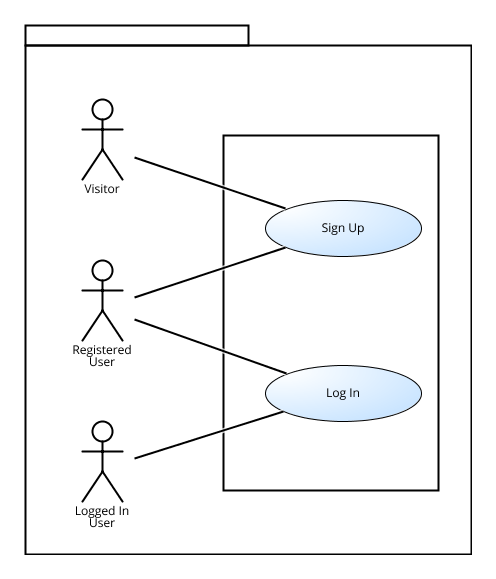
\includegraphics[scale=0.5]{Pictures/UseCaseDiagram/Log_In_System.png}
\caption{UML Use Case Diagram for Log In System}
\end{figure}

\begin{figure}[H]
\centering
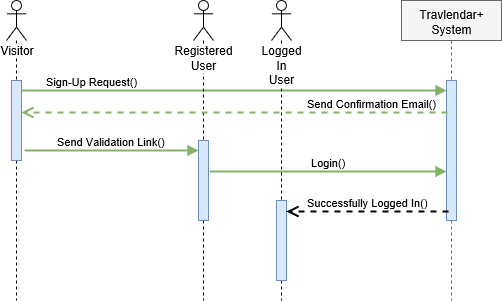
\includegraphics[scale=0.5]{Pictures/SequenceDiagram/login.png}
\caption{UML Sequence Diagram for Log In System}
\end{figure}

From this point among the next sections, we consider as the \emph{User} a logged user.